%
% OpenDCS Proposal
%
% Author: Geoff Johnson
%
% To compile: pdflatex --shell-escape --synctex=1 --interaction=nonstopmode proposal.tex
%

\documentclass[11pt]{article}

\usepackage[titles]{tocloft}
\usepackage{verbatim}
\usepackage[pdftex]{graphics,graphicx}
\usepackage[export]{adjustbox}
\usepackage{booktabs}
\usepackage{pdfpages}
\usepackage{float}
\usepackage{amssymb}
\usepackage{mathtools}
\usepackage{biblatex}
\usepackage{svg}
\usepackage{tikz}
\usetikzlibrary{arrows}
\bibliography{references}

\usepackage{hyperref}
\hypersetup{%
  pdfauthor={Geoff Johnson},
  pdftitle={OpenDCS Project Proposal},
  pdfsubject={Project Proposal},
  pdfkeywords={OpenDCS Project Proposal},
  colorlinks=true,
  linkcolor=black,
  urlcolor=blue
}

% Packages used for appendices.
\usepackage{appendix}
\usepackage{listings}
\usepackage{color}
\definecolor{light-gray}{gray}{0.95}
\definecolor{listinggray}{gray}{0.9}
\definecolor{lbcolor}{rgb}{0.9,0.9,0.9}
\definecolor{light-blue}{rgb}{0.6,0.720,0.85}

% The default margins are too wide all the way around, reset them.
\setlength{\topmargin}{-.5in}
\setlength{\textheight}{9in}
\setlength{\oddsidemargin}{0in}
\setlength{\textwidth}{6.5in}

% Change paragraph formatting.
\setlength{\parindent}{0pt}
\setlength{\parskip}{2ex}

\begin{document}
\nocite{*}

  \title{%
    Project Proposal \\
    OpenDCS - an open Distributed Control System
  }

  \author{%
    Geoff Johnson \\
    A00433581 %\\ \\
    %<course>
  }

  \renewcommand{\today}{April 1, 2016}
  \maketitle
  \thispagestyle{empty}
  \newpage
  \mbox{}
  \thispagestyle{empty}

  \newpage
  \addtocounter{page}{-1}
  \pagenumbering{roman}
  \tableofcontents
  %\listoffigures
  %\listoftables
  %\lstlistoflistings

  \newpage
  \pagenumbering{arabic}

  % XXX fill in or omit sections as needed, for now just blasting ideas

  % The institution of submission requires that this document contain
  % information about the student and company that the project is by/for.
  \section{Background}\label{sec:bg}

    \subsection{Student}\label{sec:bg-student}

      Geoff Johnson is a student of the BCIT Computer Systems Bachelor's degree.
      Prior to this he obtained a diploma of Computer Systems Technology from
      Camosun college in Victoria, as well as a diploma in Robotics and Automation
      Technology from BCIT.

      Currently Geoff works in Burnaby for the fluid mechanics research and
      development company Coanda where he is responsible for managing the IT
      operations, as well as managing and contributing to control system
      software. This software is used to interface with industrial instrumentation,
      perform automated feedback control of plant processes, and capture data
      to logs at upwards of 100,000 samples per second.

    \subsection{Company}\label{sec:bg-company}

      Coanda is an engineering research and development company specializing in
      industrial fluid dynamics and related technologies.

    \subsection{Project}\label{sec:bg-project}

      The project being proposed is to take crucial portions of the current
      measurement and control software and implement them as daemonized processes.
      This server software would be responsible for managing the control,
      logging, and data acquisition sub-processes. It will also implement a
      messaging API for setting and retrieving components of the data model,
      and a PUB/SUB socket system to allow clients to register to streamed data.

  % Helicopter view of the project meant to engage the reader.
  \section{Executive Summary}\label{sec:exec}

    % XXX fill in last

  % Describe the problem domain and issues at a high level.
  \section{Project Overview}\label{sec:desc}

    The current implementation is comprised of two software projects. The first is a
    library of objects that abstracts the data acquisition hardware as various
    types of measurement channels, it handles logging to both CSV files as well
    as databases, feedback control loop calculations using the PID (Proportional
    Integral Derivative) equation, and handles the creation of object hierarchy
    through a class builder using XML as the input. This library, libcld, is an
    open source project hosted as a git repository at http://github.org/geoffjay/libcld.

    The second piece of software, shown in Figure~\ref{fig:layout-dactl}, is an
    end user GUI application developed for the Gnome system. It interfaces with
    libcld, hereafter referred to as CLD (Control, Logging, and Data
    Acquisition), context object to provide the data necessary to update the
    interface view.

    \begin{figure}[H]
      \centering
      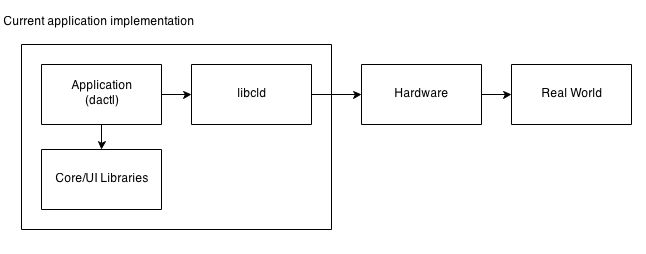
\includegraphics[scale=.6]{figures/dactl-current-layout.png}
      \caption{Current Application Design}
      \label{fig:layout-dactl}
    \end{figure}

    The proposed daemon solution is meant to address issues with the latter.
    Having high reliability tasks such as data acquisition and control reside in
    a GUI application that an unexperienced end-user operates can create reliability
    issues, sometimes through user mistakes, sometimes through issues with a
    graphical environment. A simple design of this proposed client/server
    platform is given in Figure~\ref{fig:layout-proposed-dcs}.

    \begin{figure}[H]
      \centering
      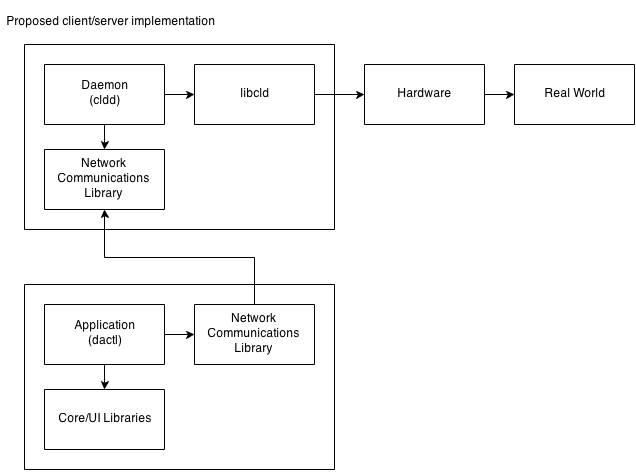
\includegraphics[scale=.6]{figures/dcs-proposed-layout.png}
      \caption{Proposed Client/Server Design}
      \label{fig:layout-proposed-dcs}
    \end{figure}

    \subsection{Scope/Domain}\label{sec:desc-domain}

      \subsubsection{Configuration Specification}\label{sec:desc-domain-conf}

      \subsubsection{Instrument Measurement}\label{sec:desc-domain-instr}

      \subsubsection{Automated Process Control}\label{sec:desc-domain-ctrl}

        % FIXME: place the figure and equation side-by-side in a box
        %\begin{figure}[htbp]
          %\centering
          %\includesvg[scale=.25,svgpath = figures/]{pid}
          %\caption{PID Control Loop}
        %\end{figure}

        \begin{equation}
          m_n = k_p*e_n + \frac{k_e*T}{T_{reset}}\sum_{i=0}^{n}e_i + k_d\frac{e_n - e_{n-1}}{\delta t} + m_{R}
        \end{equation}

      \subsubsection{Data Logging}\label{sec:desc-domain-logging}

      \subsubsection{Plugin Framework Allowing for Device Type Expansion}\label{sec:desc-domain-plugin}

  \section{Obstacles}\label{sec:obstacles}

    A project such as this which is a system of distributed components can\dots

    % XXX find a better word here than `mitigation'
    \begin{itemize}
      \item Risk: Incorrect division of necessary components \\
            Mitigation: The proposed project is largely based off of an existing set of software components, the risk
            presented here is reduced by extending and refactoring that which already works and not trying to re-invent
            anything.
      \item Risk: \\
            Mitigation:
      \item Risk: \\
            Mitigation:
    \end{itemize}

  \section{Technical Obstacles}\label{sec:tech-obstacles}

    Many of the technical obstacles presented by this project are likely going
    to be due to the desire to include unknown devices which communicate over
    different protocols and interfaces, for example RS232, I2C, TCP, SPI, etc.
    In order to address this problem directly the design and implementation of
    the underlying device library will be limited to an interface definition
    of a device modelled after a plugin, and a device loader.

    This architecture is already known to the developer and has been used in
    practice for a number of years. The device interface is a minimal
    description of what the derived plugins are capable of providing as well
    as defines what any must implement at a minimum to be understood by the
    system. For reference, this will use at an underlying level the well known
    and oft used libpeas which is included in the GNOME software ecosystem.

  % The proposed treatment to the problem described.
  \section{Proposed Solution}\label{sec:soln}

    Performing all of the work in a single application for data acquisition,
    feedback control, and data logging is open to a variety of issues. Doing so
    limits hardware scalability, places critical operations onto systems running
    desktop software, and ties high reliability functions like plant control in
    the same process as the front end that the end user operates. These are just
    to name a few of the more obvious problems.

    The system being proposed in this document is one that implements all of
    the hardware access and logging functionality into a daemon that runs as a
    process detached from the plant operator that interacts with the GUI
    application. This server software will use an existing library to interface
    with the data acquisition hardware as well as perform the control and
    logging tasks, this aspect of the software is a reimplimentation of work
    that already exists in an application that is currently in use.

    New functionality that is planned is the definition and minimal
    implementation of a REST API, a messaging system for streaming data, and a
    configuration definition to allow for the reconfiguration of the daemon. The
    REST API is meant to provide a means for clients to make simple requests of
    the system like read a single measurement value or change a property value
    of one of the internal objects. ZeroMQ is to be used to implement the
    messaging system, it has several high level features including publish and
    subscribe socket types that can be used for a streaming data system, a
    request/reply structure for a higher performance version of the REST API,
    and a structure for bridging communications to allow for the reconfiguration
    of the server as a proxy or slave node in a distributed system.

    % Discuss the benefit the end user gains from the proposed system that they
    % are currently missing.
    \subsection{Business Value}\label{sec:soln-val}

    \subsection{Development Process Model}\label{sec:soln-model}

      \subsubsection{Analysis}\label{sec:soln-model-analysis}

      \subsubsection{Design}\label{sec:soln-model-design}

      \subsubsection{Implementation}\label{sec:soln-model-implementation}

      \subsubsection{Testing}\label{sec:soln-model-testing}

        % CLD unit tests

    % Existing technologies needed to realize a solution.
    \subsection{Hardware Requirements}\label{sec:soln-tech-hw}

    \subsection{Software Requirements}\label{sec:soln-tech-sw}

      \subsubsection{ZeroMQ and Protocol Buffers for Messaging}\label{sec:soln-tech-sw-msg}

        % why use 0MQ ???
        % - protocol buffers
        % - leaves option for RDMA
        % - simple PUB/SUB implementation
        % - well documented ability to create wire protocols

      \subsubsection{Configuration and Communication Through CLD}\label{sec:soln-tech-cld}

    % XXX some other subsection ideas:
    %     - what metrics will be used to evaluate success
    %     - how will you know your objective has been met

  % Step-by-step details of the work required to achieve the proposed goal.
  \section{Work Plan}\label{sec:plan}

    \subsection{Project Timeline}\label{sec:plan-time}

      %%% XXX insert Gantt

    \subsection{Tasks \& Activities}\label{sec:plan-tasks}

      %%% XXX insert list of tasks

    \subsection{Milestones}\label{sec:plan-milestones}

      \begin{table}[H]
        \centering
        \begin{tabular}{l | p{10cm}}
          \hline
          Milestone & Description \\ [0.5ex]
          \hline\hline
          1 & something \\
          \hline
        \end{tabular}
        \caption{Project Milestones}
        \label{tab:milestones}
      \end{table}

  \section{Deployment}\label{sec:deploy}

    The project will be managed as a series of \emph{git} repositories hosted
    on \emph{github.org} using the name `OpenDCS' under an organization named
    `open-dcs', `opendcs' has unfortunately already been claimed. This
    organization and the repositories within will provide the documentation
    necessary to allow any user of the system to build from source all of the
    components. Wherever possible continuous integration will be used to
    verify the current build status of the projects, this status will be shown
    using badges in the README sections of each of the projects making it
    visible to the user what state the software is currently in.

    Realistically, reaching a stable 1.0 release of everything contained in
    this project prior to the completion date is not feasible. Part of a
    stable release would be the creation of distributable packages, eg.
    \emph{.deb/.rpm/.dmg/.msi}, for their corresponding operating systems.
    However, it may make sense at some point during development to be able
    to install the software using a package management utility in Linux and use
    an automated build system such as Copr or Launchpad to aide in the creation
    of \emph{.rpm} or \emph{.deb}. This would be an ideal deployment strategy,
    but will only be done if installation from source is for some reason deemed
    to be excessively complex.

    Another possibility for deployment would be use Docker, container software
    which is growing in popularity for simplifying in the SysOps and DevOps
    processes. Creation of a Dockerfile for each project component would not
    be a complicated addition and may happen organically during the development
    life-cycle because of what it offers towards automating testing and any
    changes in required infrastructure.

  \section{Testing}\label{sec:test}

  \section{Documentation}\label{sec:doc}

    OpenDCS will be developed as open source software and can therefore
    utilize many existing tools that offer free use to OSS projects. The
    components of the various systems will be documented using the following
    scheme:

    \begin{itemize}
      \item All software components will be hosted in an online source code
            repository system that is capable of rendering Markdown files as
            HTML, each will include sections on `Installation', `Usage',
            `Contributing', and which `License' has been used.
      \item All libraries will be developed using the Vala programming language
            and will use standard valadoc markup in the source files, API
            documentation will be generated using the tool of the same name.
      \item Any systems employing a REST API will most likely interact with an
            underlying data model, all of the documentation for the CRUD used
            by these systems will be documented along with the tool in the
            corresponding online code repository using standard Markdown format
            viewable in any web browser.
      \item The project as a whole will have a single website to pull in all of
            the associated systems, this will provide an overview of the
            project and consolidate the installation sections of each project
            into a single distilled version.
    \end{itemize}

    Examples of the documentation systems referenced:

    \begin{itemize}
      \item \href{https://help.github.com/articles/basic-writing-and-formatting-syntax/}{Markdown}
      \item \href{http://valadoc.org}{valadoc}
      \item \href{http://theforeman.org/api/1.11/index.html}{CRUD}
    \end{itemize}

  % Insert a list of references that were cited.
  \newpage
  \printbibliography%

  % Appendices
  \newpage
  \addappheadtotoc%
  \appendix
  \appendixpage%

  % Left over from a previous proposal document, edit later as needed.
  \section{Glossary of Abbreviations and Terms}\label{app:glossary}

    Commonly used terms and an explanation of them are given in
    Table~\ref{tab:glossary}, these are primarily generic computing terms.

    \begin{table}[H]
      \centering
      \begin{tabular}{l | p{10cm}}
        \toprule
        Term & Definition/Explanation \\ [0.5ex]
        \midrule
        API & Application Programming interface \\
        C & Common software programming language \\
        Client & Refers to the software application that communications with a daemon \\
        Comedi & Open source hardware drivers for Control and Measurement Devices \\
        Container & Operating system level virtualization similar to chroot jails \\
        CRUD & Create, Read, Update, Delete \\
        Daemon & Common term used to refer to a server application in a Linux system \\
        Data Acquisition & The act of gathering data from a real world process \\
        DevOps & A practice emphasizing collaboration between developers and IT professionals \\
        Docker & Container software applications used for DevOps and SysOps \\
        GLib & Standard set of Linux system libraries for the Gnome window manager \\
        GNU & A collection of applications, libraries, and developer tools \\
        Gnome & Open source dekstop environment software used with Linux systems \\
        GObject & A C type library to gain object oriented style features \\
        GUI & Graphical User Interface \\
        OSS & Open Source Software \\
        Perl & A high level programming language good for rapid development \\
        Plant & Term commonly used for industrial control systems \\
        REST & Representational State Transfer \\
        RS232 & Serial communication devices that has been ubiquitous for decades \\
        SysOps & System operator of a multi-user computing system \\
        Vala & An object oriented programming language that uses GObject types \\
        valadoc & A documentation standard and tool for creating API descriptions \\
        Watchdog & Standard concept for monitoring a vital systems heartbeat \\
        XML & Extensible markup language, common for use in messaging systems \\
        \bottomrule
      \end{tabular}
      \caption{Glossary of Terms}
      \label{tab:glossary}
    \end{table}

\end{document}
